%Präambel
\documentclass[12pt, a4paper]{article} %Dokumentenklasse: Seitenformat und Schriftgröße
\usepackage{mathptmx}
\usepackage[T1]{fontenc} %Pakete für die Zeichenbelegung und Schriftart Times New Roman
\usepackage[utf8]{inputenc} %Paket für die Zeichenkodierung (WICHTIG: auf Kodierung des Editors achten!!!)
\usepackage[german, ngerman]{babel}	%Paket für die Silbentrennung (letztgenannte Sprache ist Standard)
\usepackage{csquotes} %Paket für Anführungszeichen
\usepackage{graphics, graphicx} %Paket für die Einbindung von Grafiken
\usepackage{amssymb, amsmath, amstext} %Pakete für Formeln
\usepackage[left=2.5cm, right=4cm, top=2.5cm, bottom=2.5cm]{geometry} %Einstellung der Seitenränder
\setlength{\parindent}{0em} %kein Einzug
\usepackage[onehalfspacing]{setspace}	%Paket für die Zeilenabstände


\usepackage{url} %Paket für Hyperlinks
\usepackage{acronym} % Paket für Abkürzungen
\usepackage[breaklinks=true, linktocpage=true]{hyperref} %Software-Paket für Verlinken von Querverweisen, URLs, DOIs etc.
\hypersetup{ %modifiziere Link-Farben im Dokument
    colorlinks,
    citecolor=black,
    filecolor=blue,
    linkcolor=blue,
    urlcolor=blue
}
\usepackage{cite}

%Dokument
\begin{document}
\newgeometry{left=2cm, right=2cm, top=2.5cm, bottom=2.5cm}
\thispagestyle{empty}
\begin{center}

\includegraphics[width=6cm]{Bilder/wwu_logo.png} \hspace{1.3cm} 

\includegraphics[width=6cm]{Bilder/ifgi_logo.png}

\vspace{3cm}

Westfälische Wilhelms-Universität Münster

Institut für Geoinformatik 

\vspace{3cm}

\textbf{\large Bachelorarbeit} 

im Fach Geoinformatik
\vspace{1cm}

\textbf{\large Rich Data Interfaces for Copernicus Data}

\vspace{1cm}


Themensteller: Prof. Dr. Albert Remke\\
Betreuer: Dr. Christian Knoth, Dipl.-Geoinf. Matthes Rieke\\
Ausgabetermin: tbd.\\
Abgabetermin: tbd.\\
\vspace{0.5cm}
Vorgelegt von: Alexander Nicolas Pilz\\
Geboren: 06.12.1995\\
Telefonnummer: 0176 96982246\\
E-Mail-Adresse:	apilz@uni-muenster.de\\
Matrikelnummer: 512 269\\
Studiengang: Bachelor Geoinformatik\\
Fachsemester: 6. Semester\\

\end{center}
\pagenumbering{arabic}
\newpage
\tableofcontents 
\newpage
\listoffigures
\newpage
\input{Kapitel/Abkürzungsverzeichnis.tex}

\newpage
\restoregeometry
\section{Einleitung}
\subsection{Motivation}
?Wofür werden Geodaten über das Web gebraucht?
Geodaten werden von einer breiten Nutzerschicht für die unterschiedlichsten Anwendungsfälle benötigt.
Zu diesen Anwendungsfällen gehören unter anderem der Umwelt- und Katastropehnschutz. Dort werden flächendeckende,
verlässliche und aktuelle Geodaten benötigt. Diese müssen schnell und einfach beschaft und verarbeitet werden können
um zum Beispiel rechtzeitig Maßnahmen ergreifen oder mögliche Schäden quantifizieren. 

?Wo ist das Problem bei complexen oder rohen Geodaten?
Flächendecknde Fernerkundungsdaten von diversen Plattformen werden vom europäischen Copernicus Programm 
erfasst und im Internet bereitgestellt und können über Webseiten und APIs beschafft werden. 
Manche Daten, wie die Radardaten der Sentinel-1 Mission, bedürfen jedoch einer komplexen Vorverarbeitung befor aus ihnen verlässliche Aussagen über die in den Abgebildeten Räume 
stattfindenden Phänomene gemacht werden können. Die Vorverarbeitungen können nicht von allen Nutzern selbst durchgeführt werden. Zum einen Verfügen nicht alle Nutzer über die 
nötigen Fachkenntnisse und zum anderen stehen nicht jedem Nutzer entsprechende techniche Infrastrukturen zur Verfügung. 

?Daten Beschaffung über API??Rich Data Interfaces als Lösung?
Um dieses Probel zu lösen und Nutzer mit einsatzbereiten Geodaten oder abgeleiteten Produkten zu versorgen können sogenannte Rich Data Interfaces zum Einsatz kommen.  

?In Standardisierter Weise?
Um die Interoprabilität einer solchen Anwendung sicherzsutellen sollte diese nach den Maßgabene eines Standards implementiert werden. OGC API - Processes - Part 1: Core ist ein 
Standard nach dem APIs implementiert werden können welche als Ressource Prozesse bereitstellen. 

\subsection{Ziele}
Ziel dieser Arbeit ist beantwortung der Frage ob sich des OGC API - Processes - Part 1: Core Standards als Grundlage zur Implementierung von Rich Data Interfaces für die 
Daten des Copernicus Programmes eignet.  
Zur Klärung dieser Frage soll eine prototypische Anwendung implementiert werden. Teil dieser Anwendung soll eine API sein welche die Vorgaben des OGC API - Processes - Part 1: Core Standards 
umsetzt. Um eine Bezug zu einem realen Anwendungsszenario zu schaffen sollen Überschwemmungsmasken und der Sigam-Diffence-Sigma-Naught Index als Ressourcen über die API abfragbar sein. 
Die zur Verfügung gestellten ressourcen sollen aus Daten der Sentinel-1 Sattelitenmission abgeleitet werden.  
Zusätzlich soll die prototypische Anwendung evaluiert werden.
\subsection{Aufbau} 
-> Grundlagen zum schaffen der Grundkenntnisse
Im Implementierungsteil wird die prototypische Implementierung des Rich Data Interface für Copernicus-Daten vorgestellt. Dabei wird zunächst die verwendete Software, die Programmstruktur sowie 
grundlegende Eingenschaften der angebotenen Ressourcen erläutert. Anschließend werden die Implementierungen der umgesetzten Requirements-Classes des OGC API - Processes - Part 1: Core Standard 
sowie zusätzliche Funktionen beschrieben.
beschrieben. 
-> Evaluation durch Heuristiken und Test Suit 
-> Diskussion
Im Ausblick soll kurz umrissen werden wie eine hier prototypisch umgesetzte Anwendung weiterentwickelt werden könnte. 
Als Abschluss der Arbeit soll ein kurzes Fazit dienen welches die gewonnenen Erkenntnisse zusammenfasst. 



\newpage
\restoregeometry
\section{Grundlagen}
\subsection{Radarfernerkundung}
Bei der Radarfernerkundung werden vom Radarsystem elektromagnetische Impulse ausgesandt und deren Reflektionen, auch Backscatter genannt, empfangen und 
verarbeitet. Daher gehört die Radarfernerkundung zu den aktiven Fernerkundungsmethoden da hier im Gegensatz zur optischen Fernerkundung nicht nur 
von Oberflächen reflektierte Strahlung von anderen Strahlungsquellen wie der Sonne aufgenommen wird, sondern das Fernerkundungssystem 
selbst als Strahlungsquelle dient. Messungen können daher tageszeitunabhängig erfolgen. Dabei können die sendenden und erfangenden Komponenten unterschiedlich (bi- oder multistatisches Radar) oder 
identisch sein (monostatitsches Radar). Trifft der ausgesandte Impuls auf eine Oberfläche, zum Beispiel die Erdoberfläche, wird nur ein Teil des Signals 
reflektiert und vom Fernerkundungssystem empfangen \cite{tutorial_on_sar}. 

Die Eigenschaften dieses empfangenen Signal hängen sowohl von Parametern des Aufnahmesystems als von Parametern der reflektierenden Oberfläche ab.
So werden in der Radarfernerkundung verschiedenen Frequenzbänder verwendet, welche sich in Frequenz und Wellenlänge unterscheiden. 
Mit einer größeren Wellenlänge kann ein Medium tiefer durchdrungen werden. Außerdem werden Wolken, Dunst und Rauch durchdrungen was den zusätzlich Vorteil bietet
wetterunabhängig Messungen durchführen zu können \cite{einfuehrung_in_fernerkundung}. Gängige in der Radarfernerkundung verwendete Frequenzbänder können Tabelle x entnommen werden. 

\begin{table}[htb]
    \caption{Gängige Frequenz-Bänder in der Radarfernerkundung}
\begin{center}
    \begin{tabular}{|c|c|c|c|c|c|c|c|} 
        Frequenzband & Ka & Ku & X & C & S & L & P\\ 
        \hline
        Frequenz (GHz) & 40-25 & 17.6-12 & 12-7.5 & 7.5-3.75 & 3.75-2 & 2-1 & 0.5-0.25\\ 
        Wellenlänge (cm) & 0.75–1.2 & 1.7–2.5 & 2.5–4 & 4–8 & 8–15 & 15–30 & 60–120\\ 
    \end{tabular}
    \label{table:1}
\end{center}
\end{table}

Die Durchdringung hängt auch von der Dielektrizitätskonstante der reflektierenden Materialen ab. Ist diese groß, reflektiert die Oberfläche stark und die Durchdringung ist gering.
Zusätzlich ist die Polarisation der ausgesandten und empfangenen Signale bei der Messung ausschalgebend. Sie können horizontal oder vertikal polarisiert sein. Dies führt zu vier möglichen 
Polarisationsmodi für das Senden (transcieve) und das Empfangen (receive) nämlich HH, VV, HV und VH.
Der Depressionswinkel der Antenne nimmt direkten Einfluss auf die geometrische Auflösung quer zur Flurrichtung (Range Resolution) da dadurch die Dauer eines ausgestrahlten Signals
beeinflusst wird. Die geometrische Auflösung in Flugrichtung (Azimut Resolution) wiederum wird von der Länge der Sendeantenne und ihrem Abstrahlwinkel beeinflusst. Die Antennenlänge kann Bauartbedingt 
nicht beliebig gesteigert werden \cite{einfuehrung_in_fernerkundung}. So aufgenommene Daten haben also keine Quadratische Auflösung. Die tatsächliche Ausdehnung der Objekte quer zu Flugrichtung (Ground-Range) 
wird verzerrt wiedergegeben (Slant-Range). Die breite des Aufnahmegebietes (swath width) ist gleich der Ausdehnung der Ground-Range. Die Länge ergibt sich aus dem Zeitraum, indem das Radar eingeschaltet ist \cite{tutorial_on_sar}.

Plattformen, welche mit Radarsystemen mit synthetischer Apertur ausgerüstet sind, werden seit den 1980er Jahren als 
Mittel der Fernerkundung eingesetzt. Diese Systeme mit verhältnismäßig kurzen Antennen mit breitem Abstrahlwinkel ausgestattet. Durch die Bewegung der Plattform entlang 
des Azimuts kann die wirksame Antennenlänge (synthetisch) vergrößert und die empfangenen Signale miteinander korreliert werden um so eine hohe geometrische Auflösung zu erzielen \cite{tutorial_on_sar}\cite{einfuehrung_in_fernerkundung}.

\begin{figure}[h]
    \centering
    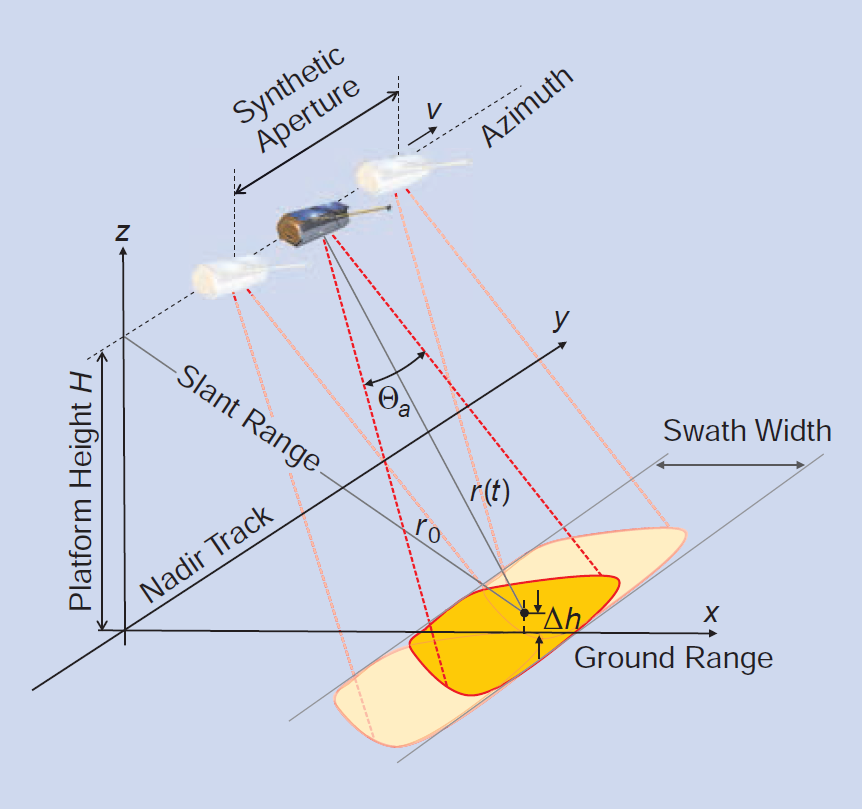
\includegraphics[width=12cm]{Bilder/SAR_Prinzip.png}
    \caption{Prinzip des Synthetic Aperture Radar - Quelle: \cite{tutorial_on_sar}}
    \label{fig:sar_prinzip}
\end{figure}

Die Rauigkeit ist eine Eigenschaft der reflektierenden Oberfläche und hat großen Einfluss auf das reflektierte Signal. Ist diese im Verhältnis zu verwandten
Wellenlänge gering so kommt es zur Spiegelung und nur ein geringer bis kein Anteil des kehrt zum Empfänger zurück. Doch auch die Form und Exposition der Oberfläche nimmt 
Einfluss auf das reflektierte Signal. So werden Flächen unterschiedlich stark bestrahlt. Ist eine dem System abgewandte Fläche steiler geneigt als der Depressionswinkel liegen Sie
sogar im Radarschatten und werden gar nicht bestrahlt \cite{einfuehrung_in_fernerkundung}. 
Im Gegensatz zu optischen Aufnahmeverfahren liefern die Rohdaten einer Befliegung mit Radarsensoren noch keine Bilddaten. Um Bilder zu erzeugen, bedarf es zunächst einer komplexen
Verarbeitung. Dabei werden die Daten entlang der Range- und Azimut-Dimension gefiltert. In der Regel repräsentieren die Pixelwerte eines aus Radardaten abgeleiteten Bildes der 
Reflektivität der korrespondierenden Fläche. Mittels Geocodierung kann das so entstandene Bild verortet werden.
Zusätzlich können diverse Kalibrierungen vorgenommen werden. Dazu gehören Verfahren welche Rauscheffekte minimieren, die geometrischen Eigenschaften verbessern oder die Interpretation
der Bilder erleichtern \cite{tutorial_on_sar}. 

\subsection{Copernicus Programm}
\subsubsection{Ziele}
\subsubsection{Sentinel 1}
\subsubsection{Datenzugang}
\subsection{Überschwemmungsmonitoring}
\subsection{Schnittstellen}
\subsection{OGC und OGC Standards}
\subsection{OGC API - Processes - Part 1: Core}
\subsubsection{Ziele}
\subsubsection{Aufbau}
\subsection{Evaluationskriterien}
\newpage
\restoregeometry
\section{Implementierung}
\subsection{Requirements Class Core}
\subsection{Requirements Class OGC Process Description}
\subsection{Requirements Class JSON}
\subsection{Requirements Class HTML}
\subsection{Requirements Class OpenAPI 3.0}
\subsection{Requirements Class Job List}
\subsection{Requirements Class Dismiss}
\subsection{Zusätzliche Funktionalitäten}
\subsection{Überschwemmungsmonitoring}
Eines dieses Schwellwertverfahren wurde von Nobuyuki Otsu entwickelt und ist nach ihm benannt. Bei diesem Verfahren werden alle Werte eines Histogramms durchlaufen.
Jeder dieser Werte teilt das Histogramm in zwei Gruppen und bildet so einen Schwellwert. Jener Wert welcher die gewichtete Varianz innerhalb der Klassen minimiert.
Gegeben sei ein Bild $C$ mit $N$ Pixeln und $L$ Grauwertstufen. Die Anzahl der Pixel einer Grauwertstufe $i$ sein dann gegeben durch $n_i$ mit:

\begin{equation}
    N = \sum_{i=1}^{L} n_i
\end{equation}
Der momentan betrachtete Grenzwert $t$ teil das Bild in die Gruppen $C_0$ und $C_1$ wobei $C_0$ alle Pixel der Graustufen 1 bis $t$ und 
$C_1$ alle Pixel der Graustufen $t+1$ bis $L$ enthält. Die Gewichte für die Gruppen $C_0$ und $C_1$ sind nun gegeben durch:
\begin{equation}
    w_0(t) = w(t) = \sum_{i=1}^{t} p_i
    \text{   und   }
    w_1(t) = \sum_{i=t+1}^{L} p_i
\end{equation}
Mit pi:
\begin{equation}
    p_i = \frac{n_i}{N}
\end{equation}
und:
\begin{equation}
    \mu_0(t) = \sum_{i=1}^{t} ip_i/w_0
    \text{   und   }
    \mu_1(t) = \sum_{i=t+1}^{L} ip_i/w_1
    \text{   und   }
    \mu_T = \sum_{i=1}^{L} ip_i
\end{equation}
Die Klassenvarianzen sind gegeben durch:
\begin{equation}
    \sigma_0^2(t) =  \sum_{i=1}^{t} (i-\mu_0)^2p_i/w_0
    \text{   und   }
    \sigma_1^2(t) = \sum_{i=t+1}^{L} (i-\mu_1)^2p_i/w_1
\end{equation}
Zu Maximieren ist nun die Inter-Klassenvarianz was equivalent zur Minimierung der Intra-Klassenvarianz ist:
\begin{equation}
    K = \frac{\sigma_t^2}{\sigma_W^2}
\end{equation}
wobei: 
\begin{equation}
    \sigma_W^2 = w_0\sigma_0^2 + w_1\sigma_1^2
    \text{   und   }
    \sigma_T^2 = \sum_{i=1}^{L} (i-\mu_T)^2p_i
\end{equation}

\newpage
\restoregeometry
\section{Evaluation}
\subsection{Jakob's Nutzbarkeitsheuristiken}
\subsection{Unit Testsuit}
\subsection{OGC Compliance Test}
\newpage
\restoregeometry
\section{Ausblick}



\newpage
\thispagestyle{empty}
\begin{thebibliography}{1}
\bibitem{s1_product_definition}
M. Bourbigot, H. Johnson, R. Piantanida. (2016, März 25). Sentinel-1 Product Definition [Online]. Verfügbar unter: 
https://sentinel.esa.int/web/sentinel/user-guides/sentinel-1-sar/document-library/-/asset\_publisher/1dO7RF5fJMbd/content/sentinel-1-product-definition 
(Zugriff am: 2. März 2022).

\bibitem{ogc_api_processes_core}
B. Pross und P. A. Vretanos. (2021, Dezember 20). OGC API – Processes – Part 1: Core [Online]. Verfügbar unter: 
https://docs.opengeospatial.org/is/18-062r2/18-062r2.html 
(Zugriff am: 1. März 2022).

\bibitem{flood_proxy_mapping_ndsi}
N. I. Ulloa, S.-H. Chiang und S.-H. Yun (2020, April 27). Flood Proxy Mapping with Normal-ized Difference Sigma-Naught Index and Shannon’s Entropy [Online]. Verfügbar unter: 
https://doi.org/10.3390/rs12091384 
(Zugriff am: 1. März 2022).

\end{thebibliography}
\input{Kapitel/Abschlusserklärung.tex}

\end{document}